\begin{figure}[htbp]
\centering
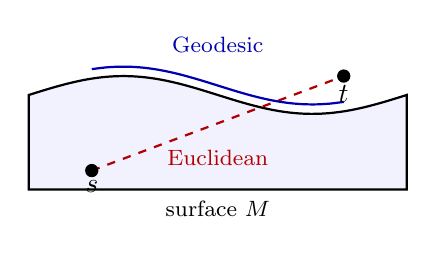
\begin{tikzpicture}[scale=0.8]
  \draw[thick,fill=blue!5] plot[smooth,domain=0:6,samples=40] (\x,{0.3*sin(\x*60)+1.5}) -- (6,0) -- (0,0) -- cycle;
  \draw[red!70!black,thick,dashed] (1,0.3) -- (5,1.8);
  \node[red!70!black,font=\footnotesize] at (3,0.5) {Euclidean};
  \draw[blue!70!black,thick] plot[smooth,domain=1:5,samples=20] (\x,{0.3*sin(\x*60)+1.5+0.15});
  \node[blue!70!black,font=\footnotesize] at (3,2.3) {Geodesic};
  \fill (1,0.3) circle (3pt) node[below] {$s$};
  \fill (5,1.8) circle (3pt) node[below] {$t$};
  \node[font=\footnotesize] at (3,-0.3) {surface $M$};
\end{tikzpicture}
\caption{Geodesic vs.\ Euclidean distance on a curved surface. The geodesic (blue) follows the terrain.}
\label{fig:geodesic}
\end{figure}
